\documentclass[review]{elsarticle}

\usepackage{lineno,hyperref}
\modulolinenumbers[5]

\journal{Journal of \LaTeX\ Templates}

%%%%%%%%%%%%%%%%%%%%%%%
%% Elsevier bibliography styles
%%%%%%%%%%%%%%%%%%%%%%%
%% To change the style, put a % in front of the second line of the current style and
%% remove the % from the second line of the style you would like to use.
%%%%%%%%%%%%%%%%%%%%%%%

%% Numbered
%\bibliographystyle{model1-num-names}

%% Numbered without titles
%\bibliographystyle{model1a-num-names}

%% Harvard
%\bibliographystyle{model2-names.bst}\biboptions{authoryear}

%% Vancouver numbered
%\usepackage{numcompress}\bibliographystyle{model3-num-names}

%% Vancouver name/year
\usepackage{numcompress}\bibliographystyle{model4-names}\biboptions{authoryear}

%% APA style
%\bibliographystyle{model5-names}\biboptions{authoryear}

%% AMA style
%\usepackage{numcompress}\bibliographystyle{model6-num-names}

%% `Elsevier LaTeX' style
\bibliographystyle{elsarticle-num}
%%%%%%%%%%%%%%%%%%%%%%%

\graphicspath{{./figure/}}

\usepackage{amsmath}
\usepackage{amssymb}
\usepackage{xeCJK}
\usepackage{enumerate}
\usepackage{amsthm}
\newtheorem{theorem}{Theorem}
\newtheorem{corollary}[theorem]{Corollary}
\newtheorem{lemma}{Lemma}
\newtheorem{example}{Example}
\newtheorem{proofOfTheorem}{Proof of Theorem}
\newtheorem{assumption}{\quad\quad Assumption}
\begin{document}

\begin{frontmatter}

\title{Integrated likelihood ratio test\tnoteref{mytitlenote}}
\tnotetext[mytitlenote]{Fully documented templates are available in the elsarticle package on \href{http://www.ctan.org/tex-archive/macros/latex/contrib/elsarticle}{CTAN}.}

%% Group authors per affiliation:
\author{author \fnref{myfootnote}}
\address{Radarweg 29, Amsterdam}
\fntext[myfootnote]{Since 1880.}

%% or include affiliations in footnotes:
\author[mymainaddress,mysecondaryaddress]{Elsevier Inc}
\ead[url]{www.elsevier.com}

\author[mysecondaryaddress]{Global Customer Service\corref{mycorrespondingauthor}}
\cortext[mycorrespondingauthor]{Corresponding author}
\ead{support@elsevier.com}

\address[mymainaddress]{1600 John F Kennedy Boulevard, Philadelphia}
\address[mysecondaryaddress]{360 Park Avenue South, New York}

\begin{abstract}

    Likelihood ratio test (LRT) is the most widely used test procedure. However, it has some weaknesses. Likelihood is unbounded for some important models. Even when the likelihood is bounded, the maximum may be not easy to obtain if it is not convex in parameters. We propose a new test procedure called integrated likelihood ratio test (ILRT) which can overcome the above difficulties. Posterior Bayes factor is a special case of ILRT\@. We proof the Wilks phenomenon of ILRT and give the asymptotic
    local power.
\end{abstract}

\begin{keyword}
%\texttt{elsarticle.cls} \sep \LaTeX \sep Elsevier \sep template
%\MSC[2010] 00-01\sep  99-00
\end{keyword}

\end{frontmatter}

%\linenumbers

\section{Introduction}

Suppose we are interested in  testing the hypotheses $H_0:\theta\in \Theta_0$ vs $H_1:\theta\in \Theta_1$. The well known LRT is defined as
\begin{equation}
    \frac{\sup_{\Theta} p_{\theta}(X)}{\sup_{\Theta_0} p_\theta(X)},
\end{equation}
where $X$ is the data, $p_\theta(X)$ is the density function of $X$ with respect to some dominating measure $\mu$.
LRT is the most widely used statistical method which enjoys many optimal properties. For example, by Neyman-Pearson lemma, it's the most powerful test (MPT) in simple null and simple alternative case.
(See~\cite{Lehmann}) In multi-dimensional parameter case, MPT does not exist. However, the LRT is asymptotic optimal in Bahadur efficiency sense. (See~\cite{MR0315820}) However, even in some widely used models, likelihood may be unbounded, see~\cite{Cam1990Maximum} for some examples.In this case,
LRT does not exist. Another weakness of LRT occurs when the likelihood is not convex in parameters. In this case, numerical algorithms for maximizing likelihood may trap in local maximum. 
To overcome these difficulties, we propose the following ILRT 

\begin{equation}
    \Lambda (X)=\frac{\int_{\Theta} p_\theta(X)\pi(\theta;X)\,d\theta}{\int_{\Theta_0} p_\theta(X)\pi^*(\theta;X)\,d\theta},
\end{equation}
where $\pi(\theta;X)$ and $\pi^*(\theta;X)$ are weight functions which may rely on data but does not need to equal to posterior density.


\cite{Aitkin1991Posterior} proposed posterior Bayes factor
\begin{equation}
    \frac{\int_{\Theta} p_\theta(X)\pi(\theta|X)\, d\theta}{\int_{\Theta_0}p_\theta(X)\pi^*(\theta|X)\, d\theta},
\end{equation}
where $p(x|\theta)$ is the sample density, $\pi^*(\theta|x)$ and $\pi(\theta|x)$ are the posterior densities under null hypotheses and alternative hypothesis.
\cite{gelfand1993bayesian} derived it's null distribution. They didn't explicitly give the conditions needed. In fact, their proof relies on Laplace approximation, which assumes the existence of maximum likelihood estimator (MLE). 
Note that if MLE exists, LRT also exists. Hence the scope of their method doesn't exceed that of classical LRT\@.



Based on the proof of Bernstein-von Mises theorem (See~\cite{van2000asymptotic} and~\cite{Kleijn2012The}), we give the proof of the Wilks phenomenon and local power of ILRT under fairly weak assumptions.

\section{Integrated likelihood ratio test}

Let $X_1,\ldots,X_n$ be a sample from distribution $P_{\theta}, \theta\in\Theta$. Denote $X=(X_1,\ldots,X_n)$. The parameter space $\Theta$ is an open subset of $\mathbb{R}^{p_2}$. The null space $\Theta_0$ is a $p_1$-dimensional subspace of $\Theta$
\begin{equation}
    \Theta_0=\{\theta\in\Theta:\theta_{p_1+1}=\theta_{0,{p_1+1}},\ldots,\theta_{p_2}=\theta_{0,{p_2}}\},
\end{equation}
where the last $p_2-p_1$ parameters $\theta_{0,{p_1+1}},\ldots,\theta_{0,{p_2}}$ are fixed. We want to test the hypothesis
\begin{equation}
H_0:\theta\in \Theta_0\quad vs. \quad H_1:\theta\in \Theta.
\end{equation}
The first $p_1$ parameters are nuisance parameters.

$\Theta_0$ can be regarded as a open subset of $\mathbb{R}^{p_1}$. To simplifies notations, we denote  $\Theta^*_0=\{{(\theta_1,\ldots,\theta_{p_1})}^T:\, (\theta_1,\ldots,\theta_{p_1},\theta_{0,p_1+1},\theta_{0,p_2})\in \Theta_0\}$. And we could use $p_1$-dimensional vector $\theta^*\in
\Theta_0^*$ to represent $\theta\in\Theta_0$ and regard $\Theta_0^*$ as null space.  Let $\pi(\theta;X)$ and $\pi^*(\theta^*;X)$ be the weight functions in $\Theta$ and $\Theta_0^*$. The integrated likelihood ratio statistic is defined as
\begin{equation}\label{likelihoodRatio}
    \Lambda (X)=\frac{\int_{\Theta} p(X|\theta)\pi(\theta;X)\,d\theta}{\int_{\Theta^*_0} p(X|\theta^*)\pi^*(\theta^*;X)\,d\theta^*}
\end{equation}


\section{Main results}

We will denote by $\rightsquigarrow$ the weak convergence. 
$dN(\mu,\Sigma)(h)$ is the density function of a normal distribution with mean $\mu$ and variance $\Sigma$.

Assume $\theta_0\in\Theta_0$ is a fixed parameter in null space. We study the asymptotic behavior of integrated likelihood ratio statistics around $\theta_0$.
Let the experiment $P_\theta : \theta\in \Theta$ be differentiable in quadratic mean at $\theta_0$. That is, there exists a vector of measurable functions $\dot{\ell}_{\theta_0}$ such that
\begin{equation}
    \int {\big[\sqrt{p_{\theta_0+h}}-\sqrt{p_{\theta_0}}-\frac{1}{2}h^T\dot{\ell}_{\theta_0}\sqrt{p_{\theta_0}}\big]}^2\, d\mu=o(\|h\|^2),\quad h\to 0,
\end{equation}
where $\mu$ is the controlling measure of $P_{\theta}$, $p_{\theta}(x)$ is the density of $P_{\theta}(x)$ relative to $\mu$ and $\dot{\ell}_{\theta_0}$ is called score function.

Let $I_{\theta_0}=P_{\theta_0}\dot{\ell}_{\theta_0}\dot{\ell}_{\theta_0}^T$ be the Fisher information matrix at $\theta_0$ and $\Delta_{n,\theta_0}=\frac{1}{\sqrt{n}}\sum_{i=1}^n I_{\theta_0}^{-1}\dot{\ell}_{\theta_0}(X_i)$ be the `locally sufficient' statistics. In null space, $\dot{\ell}^*$,$I^*_{\theta_0}$ and $\Delta_{n,\theta_0}^*$ are defined in the same way. It's easy to see that $\dot{\ell}^*_{\theta_0}$ is the first $p_1$
coordinates of $\dot{\ell}_{\theta_0}$, $I^*_{\theta_0}$ is the  first $p_1\times p_1$ submatrix of $I_{\theta_0}$ and $\Delta_{n,\theta_0}^*=\frac{1}{\sqrt{n}}\sum_{i=1}^n I_{\theta_0}^{*-1}\dot{\ell}^*_{\theta_0}(X_i)$.

Let $h=\sqrt{n}(\theta-\theta_0)$ which reparameterizes $\theta$ around $\theta_0$ by the scale of $\sqrt{n}$.  Obviously, $h=0$ under null. Under local alternatives, $h$ converges to a constant.

Listed below are the regular conditions we need:

\begin{assumption}\label{Assumption1}
    The assumptions of Bernstein-von Mises Theorem (see~\cite{van2000asymptotic} Chapter 10) are met:  $\Theta$ is a subset of $\mathbb{R}^p$. The experiment ($P_{\theta}:\theta\in\Theta$) is differentiable in quadratic mean at $\theta_0\in \Theta$ with nonsingular Fisher information matrix $I_{\theta_0}$. For every $\epsilon>0$, there exists a sequence of tests $\phi_n$ such that
        \begin{equation}
            P_{\theta_0}^n\phi_n\to 0,\quad \sup_{\|\theta-\theta_0\|\geq \epsilon} P_\theta^n(1-\phi_n)\to 0.
        \end{equation}
        Let $\pi_n(h;X)$ be a weight function satisfying 
        \begin{equation}\label{vonMisesResults}
            \|\pi_n(h;X)-dN(\Delta_{n,\theta_0},I_{\theta_0}^{-1})(h)\|\overset{P_{\theta_0}^n}{\to}0
        \end{equation}
\end{assumption}     
        
\begin{assumption}\label{Assumption2}
        For every $\epsilon>0$, there's a Lebesgue integrable function $T(h)$, a $K>0$ and a $A>0$ such that 

    \begin{equation}\label{Assump21}
    \lim_{n\to \infty}P_{\theta_0}^n(\sup_{\|h\|\geq K\sqrt{n}}(\pi_n(h;X)-T(h))\leq 0)\geq 1-\epsilon
\end{equation}

        \begin{equation}\label{Assump22}
            \lim_{n\to \infty} P_{\theta_0}^n(\sup_{\|h\|\leq K\sqrt{n}} \pi_n(h;X)\leq A)\geq 1-\epsilon
        \end{equation}
\end{assumption}

\begin{assumption}\label{Assumption3}
        There's a open neighborhood of $\theta_0$ $V$ and a measurable function $\dot{\ell}$ with $P_{\theta_0}\dot{\ell}^2<\infty$ such that, $\forall \theta_1,\theta_2\in V$,
        \begin{equation}
            |\log p_{\theta_1}(x)-\log p_{\theta_2}(x)|\leq \dot{\ell}(x)\|\theta_1-\theta_2\|.
        \end{equation}
\end{assumption}

Assumption~\ref{Assumption1} makes sure that there exists at least one weight function satisfies~\ref{vonMisesResults}, that is, the posterior density.
The condition~\ref{Assump21} assume there is a function controlling the tail of weight function. For a statistical model, the likelihood value makes no sense when $\theta$ is far away from $\theta_0$, or $\sqrt{n}h$ is large. To avoid the bad behavior of the likelihood function when $\sqrt{n}h$ is large, many theoretical works impose assumptions to likelihood. Thanks to the flexibility of weight function, we can impose~\ref{Assump21} to weight function instead. The condition~\ref{Assump22} is
satisfied in most usual case. No matter model is, condition~\ref{Assump21} and~\ref{Assump22} will be
satisfied, e.g., when 
\begin{equation}
    \pi_n(h;X)=\min(\pi_n(h|X),M) 1_{\|h\|\leq K\sqrt{n}}
\end{equation}
where $M$ and $M$ are user-specified constant and $\pi_n(h|X)$ is the posterior density.
Assumption~\ref{Assumption3} is standard in likelihood theory.

Our first theorem is
\begin{theorem}\label{theoremMain}
    Under the Assumptions $(i)$, $(ii)$ and $(iii)$. For bounded real numbers $\eta_n$, we have
    \begin{equation}
        \Big|\int_{\mathbb{R}^{p}}\frac{p_h(X)}{p_0(X)}\pi_n(h;X)\,dh-
        2^{-\frac{p}{2}}e^{\frac{1}{2}\Delta_{n,\theta_0}^T I_{\theta_0}\Delta_{n,\theta_0}}
        \Big|\xrightarrow{P_{\eta_n}^n}0
    \end{equation}
\end{theorem}


Based on Theorem~\ref{theoremMain},the asymptotic distribution of integrated likelihood ratio statistics under null hypothesis can be obtained. It can be used to determine the critical value of the test
\begin{theorem}\label{theoremWilks}
    Suppose the Assumptions of~\ref{theoremMain} are met for both $\Theta_0$ and $\Theta$,  the true parameter $\theta_0$ is an interior point of $\Theta$ and a relative interior point of $\Theta_0$, then we have
\begin{equation}
    2\log(\Lambda(X))\overset{P_0^n}{\rightsquigarrow} \chi^2_{p_2-p_1}-(p_2-p_1)\log(2)
\end{equation}

\end{theorem}

We can obtain the asymptotic distribution of the integrated likelihood ratio test under local alternatives by Le Cam's third lemma.
\begin{theorem}\label{theoremPower}
Suppose  the Assumptions of~\ref{theoremWilks} are met. The true parameter $\theta$ satisfies $\eta_n=\sqrt{n}(\theta-\theta_0)\to \eta$. If
\begin{equation}
    I_{\theta_0}=\left(
        \begin{matrix}
            I^*_{\theta_0}&I_{12}
            \\
            I_{21}&I_{22}
        \end{matrix}
    \right),
\end{equation}
$I_{22\cdot 1}=I_{22}-I_{21}I_{\theta_0}^{*-1}I_{12}$,
    then we have
\begin{equation}
    2\log(\Lambda(X))\overset{P_0^n}{\rightsquigarrow} \chi^2_{p_2-p_1}(\delta)-(p_2-p_1)\log(2)
\end{equation}
where
\begin{equation}
\delta=\eta^T
    \left(
        \begin{matrix}
            0&0\\
            0&I_{22\cdot 1}
        \end{matrix}
    \right)
    \eta
\end{equation}
\end{theorem}

The results can be explained by the limit experiment point of view. As $h_n\to h$, the `locally sufficient' statistic $\Delta_{n,\theta_0}\rightsquigarrow N(h,I^{-1}_{\theta_0})$. In the limit experiment, we have one observation $X\sim N(h,I_{\theta_0}^{-1})$. In this case, the integrated likelihood ratio test statistics can be calculated easily whose distribution is exactly the same as~\ref{theoremPower}.


\section{Normal mixture}

 Normal mixture is the first example of unbounded likelihood given in~\cite{Cam1990Maximum}. In this section, we apply ILRT to this model.


Suppose $X_1,\ldots,X_n$ are i.i.d.\ distributed as a mixture of normal distributions
\begin{equation}
    p_\theta(x)=\frac{1-\alpha}{\sqrt{2\pi}}\exp\left\{-\frac{1}{2}{(x-\mu)}^2\right\}+
    \frac{\alpha}{\sigma\sqrt{2\pi}}\exp\left\{-\frac{1}{2}\frac{{(x-\mu)}^2}{\sigma^2}\right\},
\end{equation}
 where $\alpha$ is a known constant. Suppose the parameter space is
\begin{equation}
    \Theta=\{\theta={(\mu,\sigma^2)}^T:\mu\in(\-\infty,\infty),\sigma^2\in (0,M)\},
\end{equation}
where $M$ is a sufficiently large parameter.
\cite{Cam1990Maximum} pointed out that the likelihood of the model is unbounded. In fact, let $\mu=X_1$ and let $\sigma^2\to 0$, then the likelihood tends to infinity.

Under the model, we consider testing the hypotheses $H_0:\mu=0,\sigma=2$ vs $H_1:\theta\in
\Theta$. Although LRT fails in this model, ILRT can still be used. In fact, we can verify (although cumbersome) that $(i)$, $(ii)$ and $(iii)$ all hold. Hence Theorem~\ref{theoremWilks} and~\ref{theoremPower} hold. To use ILRT, we need a weight function.
First let the weight function be the posterior density of parameters. To make the posterior density bounded from infinity, we consider the so-called zero-avoiding prior (see~\cite{bayesianDataAnalysis} section 13.2).
When $\mu=X_1$, as $\sigma^2\to 0$, the likelihood tends to infinity at the rate of ${1}/{\sigma}$. The rate can be hedged by the density of $\chi^2(3)$. Hence we adopt the following prior distribution

\begin{equation}
    dN(0,1)(\mu)\times d\chi^2(3)(\sigma^2),
\end{equation}
where $d\chi^2(3)(\sigma^2)$ represents the density of $\chi^2$ distribution with freedom $3$ taking value at $\sigma^2$. Because the $\sigma^2$ is limited in $(0,M)$, we also truncate prior of $\sigma^2$ at $M$.

We next verify the Wilks phenomenon by simulation. We take sample size $n=50,100,200$ and $\alpha=0.1,0.5,0.9$. In every combination, we repeat $1000$ samples and obtain $1000$ ILRT statistics. We expect the empirical distribution is similar to that of $\chi^2(2)$. We plot the QQ-plot of empirical distribution relative to  $\chi^2(2)$ distribution, it can be seen that ILRT can be well approximated by $\chi^2(2)$.

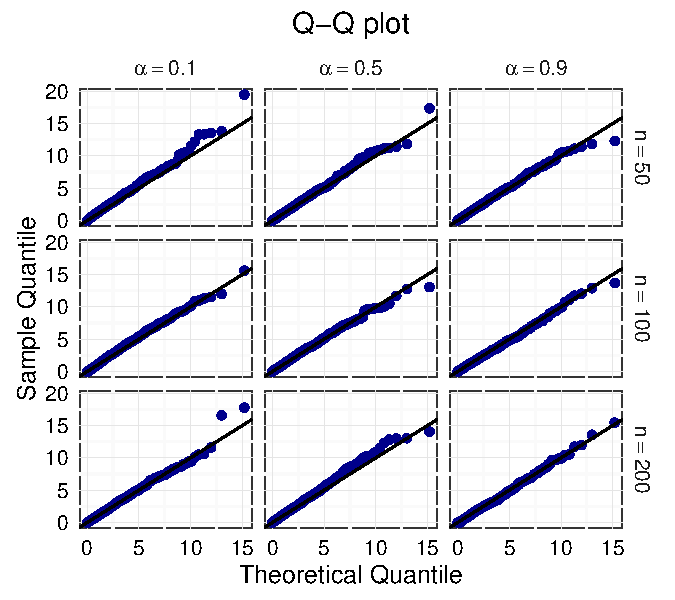
\includegraphics{myQQPlot.pdf}


We next consider another weight function $\pi (\theta; X)= N(\hat{\theta},\frac{1}{n}\hat{I}^{-1}_{\hat{\theta}})$. Lt $\hat{\theta}$ be the highest probability density estimator. And 
$$\hat{I}_\theta^{-1}=\sum_{i=1}^n
\begin{bmatrix}
-\frac{\partial^2 \log p_\theta(x_i)}{\partial \mu^2}&
    -\frac{\partial^2 \log p_\theta(x_i)}{\partial \mu\partial (\sigma^2)}
\\
    -\frac{\partial^2 \log p_\theta(x_i)}{\partial \mu\partial (\sigma^2)}
    &
    -\frac{\partial^2 \log p_\theta(x_i)}{\partial {(\sigma^2)}^2}
\end{bmatrix}$$
where

\begin{equation}
    \begin{aligned}
\frac{\partial^2 \log p_\theta(x)}{\partial
        \mu^2}=&
        \frac{(1-\alpha)({(x-\mu)}^2-1)dN(\mu,1)(x)+\alpha ({(x-\mu)}^2/\sigma^4 -\sigma^{-2})dN(\mu,\sigma^2)(x)}{p_\theta (x)}-\\
        &
        {\Big(\frac{(1-\alpha)(x-\mu)dN(\mu,1)(x)+\alpha(x-\mu)/\sigma^2 dN(\mu,\sigma^2)(x)}{p_\theta(x)}\Big)}^2,
    \end{aligned}
\end{equation}

\begin{equation}
    \begin{aligned}
        &\frac{\partial^2 \log p_\theta(x)}{\partial
        \mu\partial(\sigma^2)}=
        \frac{(\frac{3\alpha(\mu-x)}{2\sigma^4}-\frac{\alpha {(\mu-x)}^3}{2\sigma^6})dN(\mu,\sigma^2)(x)}{p_\theta (x)}-\\
        &
        \frac{\alpha (\frac{{(\mu-x)}^2}{2\sigma^4}-\frac{1}{2\sigma^2})dN(\mu,\sigma^2)(x)\big((1-\alpha)(x-\mu)dN(\mu,1)(x)+\alpha(x-\mu)/\sigma^2 d(\mu,\sigma^2)(x)\big)}{p_{\theta}{(x)}^2},
    \end{aligned}
\end{equation}


\begin{equation}
    \begin{aligned}
\frac{\partial^2 \log p_\theta(x)}{\partial
        {(\sigma^2)}^2}=&
        \frac{\alpha \big(\frac{3}{4\sigma^4}-\frac{3{(x-\mu)}^2}{2\sigma^6} +\frac{{(x-\mu)}^4}{4\sigma^8}\big)dN(\mu,\sigma^2)(x)}{p_\theta (x)}-\\
        &
        {\Big(\frac{\alpha\big(\frac{{(x-\mu)}^2}{2\sigma^4}-\frac{1}{2\sigma^2} \big)dN(\mu,\sigma^2)(x)}{p_\theta(x)}\Big)}^2.
    \end{aligned}
\end{equation}

We do the same simulation as above and the QQ-plot is given.
It  can be seen that the Wilks phenomenon still holds in this case.
For mixture model, sampling from posterior distribution is troublesome.
The computing burden will be reduce by normal approximation.
This is an advantage of normal weight ILRT.\@ From this example, we can see that ILRT is more flexible than posterior Bayes factor.


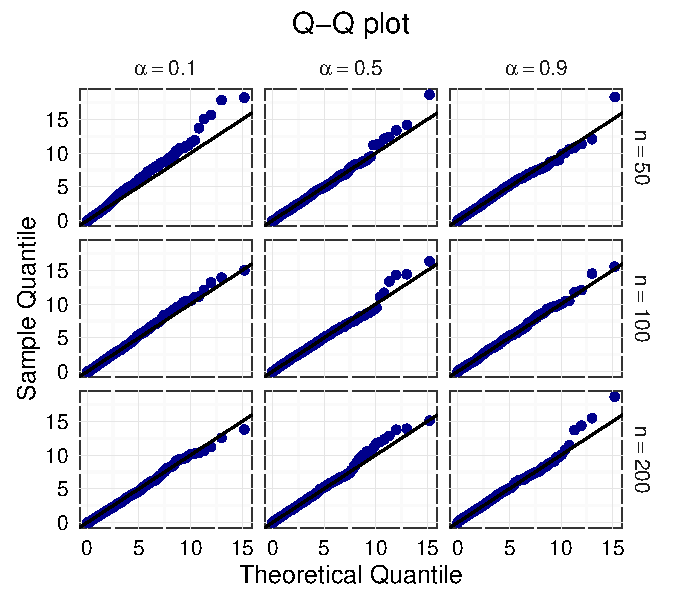
\includegraphics{myQQPlotNormal.pdf}





\section{Appendix}
For two measure sequence $P_n$ and $Q_n$ on measurable spaces $(\Omega_n,\mathcal{A}_n)$, denote by $P_n\triangleleft \triangleright Q_n$ that $P_n$ and $Q_n$ are mutually contiguous. That is, for any statistics $T_n$: $\Omega_n\mapsto \mathbb{R}^k$, we have $T_n\overset{P_n}{\rightsquigarrow}0\Leftrightarrow T_n\overset{Q_n}{\rightsquigarrow}0$.
\begin{lemma}\label{lemmaEx}
    Suppose that $\Theta$ is an open subset of $\mathbb{R}^p$ and that the model ($P_\theta: \theta \in\Theta$) is differentiable in quadratic mean at $\theta_0$. Then $P_{\theta_0}\dot{\ell}_{\theta_0}=0$ and the Fisher information matrix $I_{\theta_0}=P_{\theta_0}\dot{\ell}_{\theta_0}\dot{\ell}_{\theta_0}^T$ exists. Furthermore, for every converging sequence $h_n\to h$,as $n\to \infty$,
    \begin{equation}
        \log \frac{p^n_{h_n}(X)}{p^n_0(X)}=\frac{1}{\sqrt{n}}\sum^n_{i=1}h^T\dot{\ell}_{\theta_0}(X_i)-\frac{1}{2}h^T I_{\theta_0}h+o_{P_{\theta_0}}(1),
    \end{equation}
    where $p_h^n(X)=\prod_{i=1}^n p_h(X_i)$ is the density of $P_h^n$ relative to $\mu_n=\mu\times \cdots \times \mu$.
    (See~\cite{van2000asymptotic} Theorem 7.2.)
\end{lemma}



\begin{lemma}\label{lemmaContiguity}
    Suppose the Assumptions of Lemma~\ref{lemmaEx} are met. $U$ is a ball of fixed radius around zero. Then for every random variable sequence $T_n(X)$, $T_n\overset{P^n_0}{\rightsquigarrow}0\Leftrightarrow T_n\overset{P^n_U}{\rightsquigarrow}0$, where
\begin{equation}
    p^n_U(x)=\frac{1}{V(U)}\int_{U}p_h^n(x)dh,
\end{equation}
$V(U)$ is the volume of $U$.
\end{lemma}

\begin{proof}
In fact, we only need to prove
\begin{equation}
\int_{A_n}p_0^n(x)\, d\mu \to 0 \Leftrightarrow \int_{A_n}\frac{1}{V(U)}\int_U p_h^n(x) dh \, d\mu \to 0,
\end{equation}
or
\begin{equation}\label{eq:1}
\int_{A_n}p_0^n(x)\, d\mu \to 0 \Leftrightarrow \int_{U}\int_{A_n} p_h^n(x) d\mu \, dh \to 0.
\end{equation}
Under the assumptions of~\ref{lemmaEx}, for every bounded sequence $h_n$, $P_{h_n}^n\triangleleft \triangleright P_{0}^n$, that is
\begin{equation}\label{eq:2}
\int_{A_n}p_0^n(x)\, d\mu \to 0 \Leftrightarrow \int_{A_n} p_{h_n}^n(x) d\mu  \to 0.
\end{equation}
On the other hand, there exists sequence $\overline{h}_n$ such that
\begin{equation}
\int_{U}\int_{A_n} p_h^n(x) d\mu \, dh
\leq V(U)\sup_{h\in U}\int_{A_n} p_h^n(x) d\mu
\leq V(U)(\int_{A_n}p^n_{\overline{h}_n}(x)d\mu +1/n).
\end{equation}
 We have similar lower bound. Hence,
\begin{equation}\label{eq:3}
 V(U)(\int_{A_n}p^n_{\underline{h}_n}(x)d\mu +1/n)
\leq \int_{U}\int_{A_n} p_h^n(x) d\mu \, dh
\leq V(U)(\int_{A_n}p^n_{\overline{h}_n}(x)d\mu +1/n)
\end{equation}
The~\eqref{eq:1} follows from~\eqref{eq:2} and~\eqref{eq:3}.
\end{proof}

\begin{lemma}\label{lemmaTest}
    Suppose the assumptions of Lemma~\ref{lemmaEx} are met. Suppose that for every $\epsilon>0$ there exists a sequence of tests $\phi_n$ such that
$$
P_{\theta_0}^n \phi_n \to 0,\quad \sup_{\|\theta-\theta_0\|\geq \epsilon}P_{\theta}^n (1-\phi_n)\to 0.
$$
Then there exists for every $M_n\to \infty$ a sequence of tests $\phi_n$ and a constant $c>0$ such that, for every sufficiently large $n$ and every $\|\theta-\theta_0\|\geq M_n /\sqrt{n}$,
$$
P_{\theta_0}^n\phi_n \to 0, \quad P_\theta^n (1-\phi_n)\leq e^{-cn(\|\theta-\theta_0\|^2\wedge 1)}.
$$
    (See~\cite{van2000asymptotic} Lemma 10.3.)
\end{lemma}



\begin{lemma}\label{lemmaUniform}

    Suppose the assumptions of Lemma~\ref{lemmaEx} are met. Further more, suppose there is an open neighborhood $V$ of $\theta_0$ and a function $m(x)$ with $P_{\theta_0}m^2<\infty$ such that for all $\forall \theta_1,\theta_2\in V$:
    \begin{equation}
        |\log p_{\theta_1}(x)-\log p_{\theta_2}(x)|\leq m(x)\|\theta_1-\theta_2\|.
    \end{equation}
Then for every $M>0$,
    \begin{equation}
        \sup_{\|h\|\leq M}\Big|
         \log \frac{p^n_{h_n}(X)}{p^n_0(X)}-\frac{1}{\sqrt{n}}\sum^n_{i=1}h^T\dot{\ell}_{\theta_0}(X_i)+\frac{1}{2}h^T I_{\theta_0}h
        \Big|\xrightarrow{P^n_0}0.
    \end{equation}

    (See~\cite{van2000asymptotic} Theorem 5.23 or~\cite{Kleijn2012The} Theorem Lemma 2.1.)
\end{lemma}






\begin{proof}[\textbf{Proof of Theorem 1}]
    By contiguity,we only need to proof the convergence in $P_0^n$.

The proof consists of two steps. In the first part of the proof, let $C$ be the ball of fixed radius $M$ around zero. We proof

\begin{equation}\label{eq:14}
    \left|\int_C \frac{p^n_h(X)}{p^n_0(X)}\pi_n (h;X) \, dh-\int_C e^{h^T I_{\theta_0}\Delta_{n,\theta_0}-\frac{1}{2}h^T I_{\theta_0}h}dN(\Delta_{n,\theta_0},I_{\theta_0}^{-1})(h)\, dh\right|
 \xrightarrow{P^n_0}0
\end{equation}
By Lemma~\ref{lemmaUniform}, for every fixed $M$,
\begin{equation}
    \sup_{\|h\|\leq M}|\log \frac{p_h^n(X)}{p_0^n(X)}-h^T I_{\theta_0}\Delta_{n,\theta_0}+\frac{1}{2}h^T I_{\theta_0}h|\xrightarrow{P_0^n}0 
\end{equation}
Hence we have
\begin{equation}\label{eq:8}
    \int_C \frac{p_h^n(X)}{p_0^n(X)}\pi_n (h;X) \, dh=e^{o_{p^n_0}(1)}\int_C e^{h^T I_{\theta_0}\Delta_{n,\theta_0}-\frac{1}{2}h^T I_{\theta_0}h}\pi_n (h;X) \, dh
\end{equation}
So we only need to consider $\int_C e^{h^T I_{\theta_0}\Delta_{n,\theta_0}-\frac{1}{2}h^T I_{\theta_0}h}\pi_n (h;X) \, dh$.
    Notice that $C$ is a bounded region,hence $\Delta_{n,\theta_0}$ converges to a normal distribution. Therefore, $\sup_{h\in C}e^{h^T I_{\theta_0}\Delta_{n,\theta_0}-\frac{1}{2}h^T I_{\theta_0}h}$ is bounded in probability. So for every $\delta>0$, there exists $M$ such that, with probability $1-\delta$,
\begin{equation}
\begin{aligned}
    \int_C e^{h^T I_{\theta_0}\Delta_{n,\theta_0}-\frac{1}{2}h^T I_{\theta_0}h}|\pi_n (h;X)-dN(\Delta_{n,\theta_0},I_{\theta_0}^{-1})(h)|\, dh
\\
\leq M\int_C |\pi_n(h;X)-dN(\Delta_{n,\theta_0},I_{\theta_0}^{-1})(h)|\, dh\xrightarrow{P^n_0}0
\end{aligned}
\end{equation}
Combining with~\eqref{eq:8}, we can conclude that~\eqref{eq:14} holds. \\

This is true for every ball $C$ of fixed radius $M$ and hence also for some $M_n\to \infty$.

In the second part, we proof
\begin{equation}\label{eq:4}
    \frac{\int_{c_n^c}p_h^n(X)\pi_n(h;X)\, dh}{\int p_h^n(X)\pi_n(h;X)\, dh}\xrightarrow{P_0^n}0,
\end{equation}
where $C_n$ is a ball with radius $M_n$, for any $M_n\to \infty$.
    
    Let $\phi_n$ be the test satisfies condition $(i)$, we have

\begin{equation}
    \frac{\int_{C_n^C}p_h^n(x)\pi(h|x)\, dh}{\int p_h^n(x)\pi(h|x)\, dh}= \frac{\int_{C_n^C}p_h^n(x)\pi(h|x)\, dh}{\int p_h^n(x)\pi(h|x)\, dh}\phi_n+ \frac{\int_{C_n^C}p_h^n(x)\pi(h|x)\, dh}{\int p_h^n(x)\pi(h|x)\, dh}(1-\phi_n)
\end{equation}
Since $\eqref{eq:4}\leq 1$, 
\begin{equation}
    \frac{\int_{C_n^C}p_h^n(X)\pi_n(h;X)\, dh}{\int p_h^n(X)\pi_n(h;X)\, dh}\phi_n\leq \phi_n\xrightarrow{P_0^n}0
\end{equation}
It's enough to proof
\begin{equation}\label{eq:10}
    \frac{\int_{C_n^C}p_h^n(X)\pi_n(h;X)\, dh}{\int p_h^n(X)\pi_n(h;X)\, dh}(1-\phi_n)\xrightarrow{P_0^n}0
\end{equation}
Fix a ball $U$ around zero. Then
\begin{equation}\label{eq:11}
\eqref{eq:10}\leq \frac{\int_{C_n^C}p_h^n(X)\pi_n(h;X)\, dh}{\int_U p_h^n(X)\pi_n(h;X)\, dh}(1-\phi_n)
\end{equation}

    By the Assumption (ii) and the fact that $\Delta_{n,\theta_0}$ is uniformly tight, we can assume $\sup_h (\pi_n(h;X)-T(h))\leq 0$ and $|\Delta_{n,\theta_0}|\leq M$ for some $M$ without loss of generality since the probability they don't hold will be eventually smaller than any prespecified constant. 

    %由条件$(ii)$,给定$\delta$,当$n$充分大时,以概率$1-\delta$有$\pi_n(h;X)<A$($\forall h\in U$)。 给定$\delta_1$, 则$M_{\delta_1}$ 使得当$n$充分大时,以概率$1-\delta_1$有$|\Delta_{n,\theta_0}|<M_{\delta_1}$。
    There exists an $m>0$ such that
\begin{equation}
    \inf_{h\in U} dN(\Delta_{n,\theta_0},I_{\theta_0}^{-1})(h)\geq m.
\end{equation}
Let $D_n(X)$ be the set $\{h: |\pi_{n}(h;X)-n(\Delta_{n,\theta_{0}},I_{\theta_{0}}^{-1})|\geq\frac{m}{2}\}$. We have
%再注意到$\pi_n(h;X)$的支撑在$\{h:\|h\|\leq K\}$上。所以我们以概率$1-\delta-\delta_1$有
\begin{equation}\label{eq:13}
    \begin{aligned}~\eqref{eq:11}\leq&\frac{\int_{C_n^C}p_h^n(X)\pi_n(h;X)\, dh}{\int_{U/D_n(X)} p_h^n(X)\pi_n(h;X)\, dh}(1-\phi_n)\\
        \leq&\frac{\int_{C_n^C}p_h^n(X)\pi_n(h;X)\, dh}{\frac{m}{2}\int_{U/D_n(X)} p_h^n(X)\, dh}(1-\phi_n)\\
    \end{aligned}
\end{equation}
Next we proof
\begin{equation}\label{eq:12}
    \frac{\int_{U/D_n(X)} p_h^n(X)\, dh}{\int_U p_h^n(X)\, dh}\xrightarrow{P_0^n}1.
\end{equation}
By Assumption $(i)$, Bernstein-von Mises Theorem holds. That is
\begin{equation}\label{eq:9}
 \int |\pi_{n}(h;X)-n(\Delta_{n,\theta_{0}},I_{\theta_{0}}^{-1})|\, dh\xrightarrow{P_0^n}0   
\end{equation}
\eqref{eq:9} implies $\int 1_{D_n(x)}\, dh\xrightarrow{P_0^n}0$. Similar to the proof in step 1, we have

\begin{equation}
\begin{aligned}~\eqref{eq:12}&=\frac{\int_{U/D_n(X)} \frac{p_h^n(X)}{p_0^n(X)}\, dh}{\int_U \frac{p_h^n(X)}{p_0^n(X)}\, dh}\\
                 &=\frac{e^{o_{P^n_0}(1)}\int_{U/D_n(X)} e^{h^T I_{\theta_0}\Delta_{n,\theta_0}-\frac{1}{2}h^T I_{\theta_0}h} \, dh}{e^{o^n_{P_0}(1)}\int_U e^{h^T I_{\theta_0}\Delta_{n,\theta_0}-\frac{1}{2}h^T I_{\theta_0}h} \, dh}\\
                 &\xrightarrow{P_0^n} 1
\end{aligned}
\end{equation}
since $h^T I_{\theta_0}\Delta_{n,\theta_0}-\frac{1}{2}h^T I_{\theta_0}h$ is bounded.


Now, to obtain $\eqref{eq:13}\xrightarrow{P_0^n}0$, we only need to prove
\begin{equation}\label{eq:5}
    \begin{aligned}
        \frac{\int_{C_n^C}p_h^n(X)(A\textbf{1}_{M_n\leq \|h\|\leq K\sqrt{n}}+T(h)\textbf{1}_{\|h\|> K\sqrt{n}})\, dh}{\int_U p_h^n(X)\, dh}(1-\phi_n)\xrightarrow{P_0^n} 0
    \end{aligned}
\end{equation}
By Lemma~\ref{lemmaContiguity}, we only need to prove $\eqref{eq:5}\xrightarrow{P_U^n}0$. To prove that, we only need to prove $\eqref{eq:5}\xrightarrow{L^1_{P_U^n}}0$, that is 
\begin{equation}\label{eq:6}
    \int \frac{\int_{C_n^C}p_h^n(x)(A\textbf{1}_{M_n\leq \|h\|\leq K\sqrt{n}}+T(h)\textbf{1}_{\|h\|> K\sqrt{n}})\, dh}{\int_U p_h^n(x)\, dh}(1-\phi_n)\big(\int_U p_h^n(x)dh\big) \, d\mu  \to 0
\end{equation}
We note that
\begin{equation}\label{eq:7}~\eqref{eq:6}=\int_{C_n^C} \Big(\int (1-\phi_n)p_h^n(x)d\mu\Big) (A\textbf{1}_{M_n\leq \|h\|\leq K\sqrt{n}}+T(h)\textbf{1}_{\|h\|> K\sqrt{n}})\, dh 
\end{equation}
By Lemma~\ref{lemmaTest}, there automatically exist tests $\phi_n$  such that for sufficiently large $n$ and $\|h\|\geq M_n$,
\begin{equation}
\int (1-\phi_n)p^n_h(x)d\mu\leq e^{-c(\|h\|^2\wedge n)}
\end{equation}
If $K< 1$, then $\|h\|^2\wedge n\geq \|h\|^2\wedge K^2n$. If $K\geq 1$, then
\begin{equation}
    \|h\|^2\wedge n=\frac{1}{K^2}(K^2\|h\|^2\wedge K^2n)\geq \frac{1}{K^2}(\|h\|^2\wedge K^2n)
\end{equation}
Let $c^*=c\min(1,1/K^2)$, then
\begin{equation}
\int (1-\phi_n)p^n_h(x)d\mu\leq e^{-c^*(\|h\|^2\wedge K^2n)}
\end{equation}
Splitting the integral into the domains $M_n\leq \|h\|\leq K\sqrt{n}$ and $\|h\|\geq K\sqrt{n}$, we see that
\begin{equation}~\eqref{eq:7}\leq \int_{\|h\|\geq M_n}e^{-c^*\|h\|^2}\, dh + e^{-c^*K^2n}\int_{\|h\|>K\sqrt{n}} T(h)\, dh  \to 0
\end{equation}
Finally we have
\begin{equation}
    \begin{aligned}
        &\left|\int \frac{p_h(X)}{p_0(X)}\pi_n (h;X) \, dh-2^{-\frac{p}{2}}e^{\frac{1}{2}\Delta_{n,\theta_0}^T I_{\theta_0}\Delta_{n,\theta_0}}
 \right|\\
        &=\left|\int \frac{p_h(X)}{p_0(X)}\pi_n (h;X) \, dh-\int_{C_n} \frac{p_h(X)}{p_0(X)}\pi_n (h;X) \, dh\right|\\
        &+\left|\int_{C_n} \frac{p_h(X)}{p_0(X)}\pi_n (h;X) \, dh -\int_{C_n} e^{h^T I_{\theta_0}\Delta_{n,\theta_0}-\frac{1}{2}h^T I_{\theta_0}h}dN(\Delta_{n,\theta_0},I_{\theta_0}^{-1})(h)\, dh\right|\\
        &+\left| \int_{C_n} e^{h^T I_{\theta_0}\Delta_{n,\theta_0}-\frac{1}{2}h^T I_{\theta_0}h}n(\Delta_{n,\theta_0},I_{\theta_0}^{-1})\, dh-2^{-\frac{p}{2}}e^{\frac{1}{2}\Delta_{n,\theta_0}^T I_{\theta_0}\Delta_{n,\theta_0}}
 \right|\\
        &=J_1+J_2+J_3
\end{aligned}
\end{equation}
By the first step of the proof, we have $J_2\xrightarrow{P^n_0}0$. Hence $\int_{C_n} \frac{p_h(X)}{p_0(X)}\pi_n (h;X) \, dh $ is bounded in probability. Therefore
\begin{equation}
\begin{aligned}
    J_1&=\int_{C_n} \frac{p_h(X)}{p_0(X)}\pi_n (h;X) \, dh\left|\frac{\int \frac{p_h(X)}{p_0(X)}\pi_n (h;X) \, dh}{\int_{C_n} \frac{p_h(X)}{p_0(X)}\pi_n (h;X) \, dh}-1\right|\\
       &=O_{P_0^n}(1)o_{P_0^n}(1)
\end{aligned}
\end{equation}
And $J_3$ convenges to $0$ for trivial reasion.
\end{proof}


\begin{proof}[\textbf{Proof of Theorem 2}]
    If the null hypothesis is true, the true parameter $\theta_0$ is an interior point of $\Theta$ and $\theta_0$ is a relative interior point of $\Theta_0$. Then we can apply Theorem~\ref{theoremMain} to both the numerator and denominator of integrated likelihood ratio statistics with $\eta_n=0$. By CLT,

    \begin{equation}
    I_{\theta_0}\Delta_{n,\theta_0}=\frac{1}{\sqrt{n}}\sum^n_{i=1}\dot{\ell}_{\theta_0}(X_i)\overset{P_0^n}{\rightsquigarrow }\xi, 
\end{equation}
where $\xi\sim N(0,I_{\theta_0})$.
\begin{equation}
    I^*_{\theta_0}\Delta^*_{n,\theta_0}=\frac{1}{\sqrt{n}}\sum^n_{i=1}\dot{\ell}^*_{\theta_0}(X_i)\overset{P_0^n}{\rightsquigarrow} \xi^*, 
\end{equation}
where $\xi^*$ is the first $p_1$ coordinates of $\xi$. Hence


\begin{equation}\label{equationNull}
    \begin{aligned} 
        \Lambda(X)&=
        \frac{2^{-\frac{p_2}{2}}\exp\{\frac{1}{2}\Delta_{n,\theta_0}^T I_{\theta_0}\Delta_{n,\theta_0}\}+o_{P_0^n}(1)
        }{2^{-\frac{p_1}{2}}\exp\{\frac{1}{2}\Delta_{n,\theta_0}^{*T}I^*_{\theta_0}\Delta^*_{n,\theta_0}\}+o_{P_0^n}(1)
        }
        \\
        &\overset{P_{0}^n}{\rightsquigarrow }
        \frac{2^{-\frac{p_2}{2}}\exp\{\frac{1}{2}\xi^T I^{-1}_{\theta_0}\xi\}
        }{2^{-\frac{p_1}{2}}\exp\{\frac{1}{2}\xi^{*T}I^{*-1}_{\theta_0}\xi^*\}
        }.
    \end{aligned}
\end{equation}
But
\begin{equation}\label{equationXi}
    \xi^T I^{-1}_{\theta_0}\xi -\xi^{*T}I^{*-1}_{\theta_0}\xi^*
    ={(I_{\theta_0}^{-\frac{1}{2}}\xi)}^T\Big(
        I_{p_{2}\times p_{2}}-
        I_{\theta_0}^{\frac{1}{2}}
        \left(\begin{matrix} 
                I^{*-1}_{\theta_0}&0\\
                0&0
        \end{matrix}\right)
        I_{\theta_0}^{\frac{1}{2}}
    \Big)(I_{\theta_0}^{-\frac{1}{2}}\xi).
\end{equation}
    $I_{\theta_0}^{-\frac{1}{2}}\xi$ is a $p_2$-dimensional standard normal distribution, The middle term is a projection matrix with rank $p_2-p_1$. Hence we have
\begin{equation}
    2\log(\Lambda(X))\overset{P_0^n}{\rightsquigarrow} \chi^2_{p_2-p_1}-(p_2-p_1)\log(2).
\end{equation}
\end{proof}

\begin{proof}[\textbf{Proof of Theorem 3}]
    We note that $h_n=\eta_n$ converges to $\eta$. By differentiability in quadratic mean, Lemma~\ref{lemmaEx} and CLT,
\begin{equation}
    \begin{aligned}
    \left(
    \begin{matrix}
        \frac{1}{\sqrt{n}}\sum^n_{i=1}\dot{\ell}_{\theta_0}(X_i)
        \\
        \log \frac{p_{\eta_n}(X)}{p_0(X)}
    \end{matrix}
    \right)
    &=\left(
        \begin{matrix}
        \frac{1}{\sqrt{n}}\sum^n_{i=1}\dot{\ell}_{\theta_0}(X_i)
        \\
        \frac{1}{\sqrt{n}}\sum^n_{i=1}\eta^T\dot{\ell}_{\theta_0}(X_i)-\frac{1}{2}\eta^T I_{\theta_0}\eta
        \end{matrix}
    \right)
    +o_{P_0^n}(1)\\
    &\overset{P_0^n}{\rightsquigarrow}
    N(
    \left(
    \begin{matrix}
        0\\
        -\frac{1}{2}\eta^T I_{\theta_0}\eta
    \end{matrix}
    \right),
    \left(
        \begin{matrix}
            I_{\theta_0}&I_{\theta_0}\eta\\
            \eta^T I_{\theta_0}&\eta^T I_{\theta_0}\eta
        \end{matrix}
    \right)
    ).
    \end{aligned}
\end{equation}
Hence by Le Cam's third lemma,
\begin{equation}
    \frac{1}{\sqrt{n}}\sum^n_{i=1}\dot{\ell}_{\theta_0}(X_i)\overset{P^n_{\eta_n}}{\rightsquigarrow}\xi\sim N(I_{\theta_0}\eta,I_{\theta_0}).
\end{equation}
By Theorem~\ref{theoremMain}, under $P_{\eta_n}^n$, we have~\eqref{equationNull}.
Hence
\begin{equation}
    2\log(\Lambda(X))\overset{P_{\eta_n}^n}{\rightsquigarrow} \chi^2_{p_2-p_1}(\delta)-(p_2-p_1)\log(2),
\end{equation}
where noncentral parameter $\delta$ can be obtained by substituting $\xi$ by $I_{\theta_0}\eta$ in~\eqref{equationXi}:
\begin{equation}
    \begin{aligned}
        \delta&=\eta^T(
        I_{\theta_0}-
        I_{\theta_0}
        \left(\begin{matrix} 
                I^{*-1}_{\theta_0}&0\\
                0&0
        \end{matrix}\right)
        I_{\theta_0}
    )\eta
    \\
    &=\eta^T
    \left(
        \begin{matrix}
            0&0\\
            0&I_{22\cdot 1}
        \end{matrix}
    \right)
    \eta.
    \end{aligned}
\end{equation}
\end{proof}



\section*{References}

\bibliography{mybibfile}


\end{document}
